\documentclass[a4paper,12pt]{article}

\usepackage[slovene]{babel}
\usepackage{amsfonts,amssymb,amsmath, mathtools}
\usepackage[utf8]{inputenc}
\usepackage[T1]{fontenc}
\usepackage{lmodern}
\usepackage{graphicx}


\def\R{\mathbb{R}} % mnozica realnih stevil

\def\qed{$\hfill\Box$}   % konec dokaza
\def\qedm{\qquad\Box}   % konec dokaza v matematičnem načinu
\newtheorem{izrek}{Izrek}
\newtheorem{trditev}{Trditev}
\newtheorem{posledica}{Posledica}
\newtheorem{lema}{Lema}
\newtheorem{pripomba}{Pripomba}
\newtheorem{definicija}{Definicija}
\newtheorem{zgled}{Zgled}


\title{Krožnica v racionalni Bezierjevi obliki \\ 
\Large Seminar pri predmetu RPGO}
\author{Samo Kralj, Anja Kišek \\
Fakulteta za matematiko in fiziko}
\date{januar 2019}

\begin{document}
%%%%%%%%%%%%%%%%%%%%%%%%%%%%%%%%%%%%
\maketitle
\section{Uvod}
V seminarski nalogi bova predstavila racionalne Bezierjeve krivulje ter njihovo uporabo pri risanju krožnic in krožnih lokov. Za razliko od polinomskih Bezierjevih krivulj, ki krožni lok lahko le poljubno dobro aproksimirajo, ga racionalne krivulje opišejo eksaktno. Pri njihovi obravnavi se je zavoljo implementacije in uporabe koristno osredotočiti na pozitivnost uteži krivulje, zato se bova poskušala omejiti le na primere, kjer se to da doseči.

V prvem poglavju bova predstavila racionalne Bezierjeve krivulje ter nekaj njihovih lastnosti. Drugo poglavje bo namenjeno konstrukciji sklenjene krožnice s pomočjo racionalne krivulje čim nižje stopnje, v tretjem pa bova ugotovljeno aplicirala na primeru krožnih lokov s pozitivnimi utežmi. Zadnje poglavje bo opisovalo uporabo izpeljanega na kubičnih polkrogih ter podalo geometrijsko konstrukcijo pripadajočega kontrolnega poligona.

\section{Racionalne Bezierjeve krivulje}
Racionalna Bezierjeva krivulja $C(t)$ stopnje $n$ v $\mathbb{R}^d$ je projekcija polinomske Bezierjeve krivulje $\tilde{C}(t)$stopnje $n$ v $\mathbb{R}^{d+1}$ na hiperravnino $w=1$, kjer je točka v $\mathbb{R}^{d+1}$ označena z $
\begin{bmatrix} x \\ w \end{bmatrix}.$ Racionalna B. krivulja stopnje $n$ je tako podana s predpisom
$$r(t) = \frac{\sum_{i=0}^n w_ib_iB_i^n(t)}{\sum_{i=0}^n w_iB_i^n(t)}, $$
kjer je $B_i^n(t)$ i-ti Bernsteinov bazni polinom stopnje $n$, $b_i$ kontrolne točke krivulje, $w_i$ pa uteži.

Racionalna krivulja $C(t) = (X(t), Y(t))$ lahko eksaktno opiše krožnico kot projekcijo krivulje
$\tilde{C}(t) = (\tilde{X}(t), \tilde{Y}(t), W(t)),$ ki leži na stožcu $$\tilde{X}(t)^2 + \tilde{Y}(t)^2 - W(t)^2 = 0,$$ na ravnino $w = 1$. Slednje nam pokaže naslednji račun:

\begin{align*}
X(t)^2 + Y(t)^2 &= 1 \\
\Big{(}\frac{\tilde{X}(t)}{W(t)}\Big{)}^2 + \Big{(}\frac{\tilde{Y}(t)}{W(t)}\Big{)}^2 &= 1\\
\tilde{X}(t)^2 + \tilde{Y}(t)^2 - W(t)^2 &= 0
\end{align*}
Prva enačba predstavlja enačbo krožnice v prostoru $\mathbb{R}^2$, nato pa koordinate točk zamenjamo za tiste iz prostora $\mathbb{R}^3$, dobljene s projekcijo na ravnino $w=1$. Izraz lahko preoblikujemo v zadnjo enačbo, ki podaja običajno enačbo stožca.

\begin{figure}[h!]
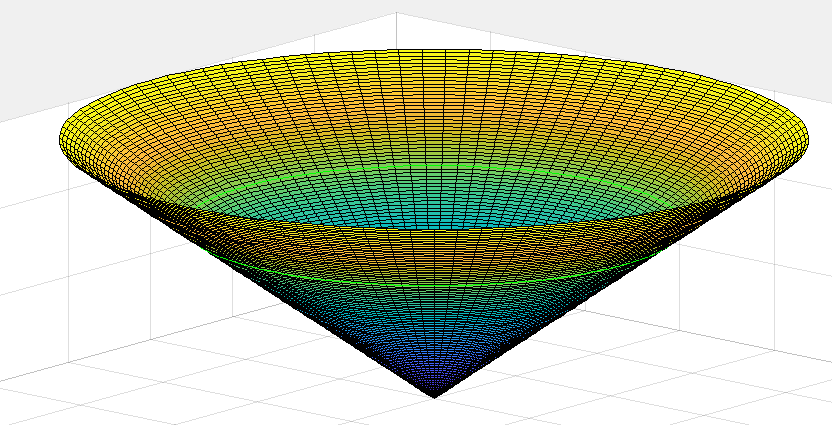
\includegraphics[scale=0.3]{stozec.png}
\centering
\caption{Stožec $\tilde{X}(t)^2 + \tilde{Y}(t)^2 - W(t)^2 = 0$, s katerega se vse krivulje projicirajo na krožnico v ravnini $w=1$.}
\end{figure}

Problem iskanja racionalne krivulje, ki opiše krožnico oziroma krožni lok, lahko prevedemo na iskanje krivulje, ki leži na omenjenem stožcu. Pogoj pozitivnih uteži lahko geometrijsko interpretiramo kot pogoj, da kontrolni poligon leži v zgornji polravnini $w > 0$.

\section{Bezierjeva krivulja kot sklenjena krivulja}
V tem poglavju si bomo ogledali, kako krožnico opišemo z eno samo racionalno krivuljo (in ne zlepkom krivulj) ter kakšna je najmanjša stopnja krivulje, s katero to lahko dosežemo.





\end{document}